\section{Modelos projetados}

~~~~~Neste capítulo são apresentadas a modelagem para as plantas, especificações e controle modular para o processo industrial de manufatura observado e estudado.

\subsection{Plantas}

~~~Os robôs 1 e 2 possuem comportamentos similares, em que as rotinas de posicionamentos espaciais são projetadas em forma de funções, as quais são acionadas por meio de sinais provenientes do Controlador Lógico Programável (CLP). 

Os movimentos e funções que o robô 1 exerce consistem nas seguintes operações:

\begin{enumerate}
	\item Pegar uma peça na mesa centralizadora: operação a qual na prática é identificada como um conjunto de movimentos que levará o robô até a posição na mesa em que as chapas metálicas estão localizadas. Após chegar nessa posição, o robô aciona as garras formadas por ventosas para pegar a peça e ao identificar que a peça foi pega, esse começa o movimento de retorno;
	
	\item Retornar da mesa centralizadora: quando o robô 1 está em uma posição segura (definida como a posição incial do robô) após voltar da mesa centralizadora, esse envia um sinal ao CLP indicando que já está com a peça e pode seguir para a próxima operação;
	
	\item Inserir a peça na prensa 1: quando o robô 1 tem uma peça e está na posição segura, ele pode inserir a peça na prensa 1, e similarmente a primeira operação será realizado um conjunto de movimentos até chegar na posição espacial da prensa 1. Assim que o robô chega na prensa as garras formadas por ventosas liberam a peça para o trabalho da prensa;
	
	\item Retornar da prensa 1: após o retorno do robô 1 da posição espacial da prensa 1 para uma posição segura, um sinal é enviado ao CLP para liberar o processo de trabalho da prensa 1;
	
	\item Em todos os estados é permitido a ocorrência de eventos de interrupção, o retorno após uma interrupção o leva para um estado inicial seguro.
\end{enumerate}

Para o robô 2, aplicam-se os mesmos princípios de operação do robô 1, porém o diferencial entre eles é o local de remoção e inserção da peça. Sendo assim, o robô 2 vai pegar a peça na prensa 1 após essa atingir o ponto motor superior (PMS). Já com a posse da peça, o robô 2 irá retornar a posição segura e quando liberado vai inserir a peça na prensa 2. Após isso, esse retorna para a posição segura.

Os modelos para a planta dos robôs 1 e 2 são apresentados na Figura \ref{fig:robo12}, onde são mostrados os eventos responsáveis pela transição de estados dos robôs. Vale destacar o fato de haver eventos de interrupção para os robôs 1 e 2, denominados por $Int\_R1$ e $Int\_R2$, respectivamente. Essas interrupções podem ocorrer devido alguma problema de reparo em algum componente da planta ou por violações de segurança da área restrita para o funcionamento dessa. Portanto, caso ocorra um evento de interrupção, os eventos que permite a volta do funcionamento dos robôs 1 e 2 foi, respectivamente, denominados por $Ret\_R1$ e $Ret\_R2$, fazendo com que os robôs voltem ao estado seguro inicial.

\begin{figure}[H]%
	\centering
	\begin{subfigure}[b]{0.45\textwidth}
		\centering
		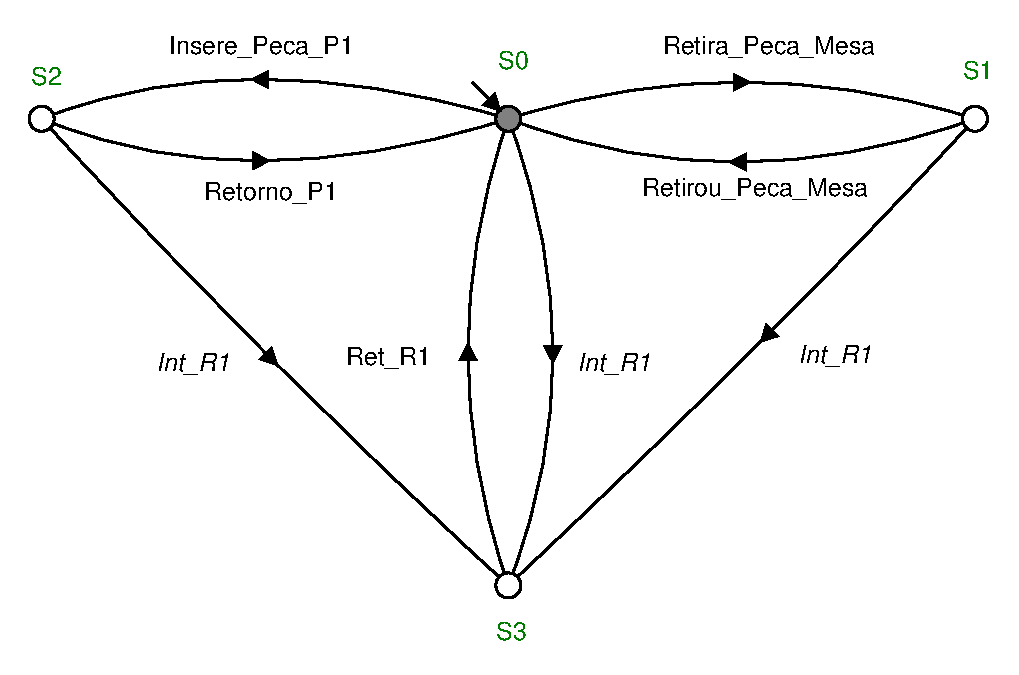
\includegraphics[width=\textwidth]{imagens/Robo_1.eps}
		\caption{Robô 1}
		\label{fig:robo1}
	\end{subfigure}
	\hfill
	\begin{subfigure}[b]{0.45\textwidth}
		\centering
		\includegraphics[width=\textwidth]{imagens/Robo_2.eps}
		\caption{Robô 2}
		\label{fig:robo2}
	\end{subfigure}
	\caption{Plantas dos robôs 1 e 2.}
	\label{fig:robo12}
\end{figure}

O robô 3 possui as mesmas rotinas de operações que o robô 2, porém na prática assim que esse retirar uma peça da prensa 2, ele precisará fazer o descarte dos retalhos da peça. Essa operação é feita internamente, então assim que esse retira a peça da prensa 2, vai até a posição do descarte, liberando as ventosas que seguram os retalhos. Após feito o descarte, o robô 3 vai para a posição segura e segue a operação, quando liberado, para inserir a peça na prensa 3. 

O modelo da planta do robô 3 é mostrado na Figura \ref{fig:robo3}, na qual estão identificados os eventos responsáveis pela transição de estados no robô 3. Novamente o evento de interrupção aparece, agora para o robô 3 e é identificado por $Int\_R3$, assim como o evento $Ret\_R3$ de retorno para o estado inicial seguro. Portanto, todos cada um dos robôs irá possuir seu evento de interrupção e retorno para estado inicial seguro.

O robô 4 possui uma rotina de operação que difere dos robôs anteriores, uma vez que esse não insere peça em uma prensa. O robô em questão leva a peça que retirou até o robô 5, uma vez que na última operação de trabalho sobre a peça, essa deve estar invertida ao ser inserida na prensa 4. Logo, o robô 4 possui as seguintes operações:

\begin{enumerate}
	\item Remover peça da prensa 3: o robô 4 a partir da sua posição segura, irá até a prensa 3 retirar a peça;
	
	\item Retornar para uma posição segura: uma vez que o robô 4 pegou a peça na prensa 3, ele retorna para a posição segura aguardando o próximo comando do CLP;
	
	\item Levar a peça para o robô 5: o robô 4 entrega a peça já invertida para o robô 5;onde ele só pode retornar assim que o robô 5 mandar sinal que já pegou a peça; 
	
	\item Retornar para a posição segura: após entregar a peça para o robô 5, o robô 4 retornará para a posição segura;
	
	\item Em todos os estados é permitido a ocorrência de evento de interrupção, o retorno da interrupção leva para um estado seguro inicial.
\end{enumerate}

O modelo da planta do robô 4 é apresentado na Figura \ref{fig:robo4}, onde são mostrados os eventos responsáveis pela transição de estados do respectivo robô.

\begin{figure}[H]%
	\centering
	\begin{subfigure}[b]{0.45\textwidth}
		\centering
		\includegraphics[width=\textwidth]{imagens/Robo_3.eps}
		\caption{Robô 3}
		\label{fig:robo3}
	\end{subfigure}
	\hfill
	\begin{subfigure}[b]{0.45\textwidth}
		\centering
		\includegraphics[width=\textwidth]{imagens/Robo_4.eps}
		\caption{Robô 4}
		\label{fig:robo4}
	\end{subfigure}
	\caption{Plantas dos robôs 3 e 4.}
	\label{fig:robo34}
\end{figure}

Como descrito anteriormente, o robô 5 é responsável por pegar a peça do robô 4 e, inserir e remover a peça na última prensa do processo industrial. As rotinas do robô 5 são apresentadas a seguir:

\begin{enumerate}
	\item Pegar peça do robô 4: após receber um sinal do CLP de que o robô 4 está posicionado com a peça pronta para ser levada para a próxima prensa, o robô 5 irá até ele para pegar a peça;
	
	\item Inserir a peça na prensa 4: com a peça capturada, o robô 5 vai inserir a peça na prensa 4 e retornar para a posição segura para que a prensa possa realizar o trabalho;
	
	\item Retirar a peça da prensa 4: após a prensa 4 finalizar o trabalho na peça, o robô 5 vai remover a peça dessa prensa e lubrificar a prensa para a próxima peça;
	
	\item Depositar a peça na esteira: uma vez com a peça retirada da prensa 4, o robô levará a peça até uma esteira onde é feito o descarte da mesma;
	
	\item Em todos os estados é permitido a ocorrência de evento de interrupção, o retorno da interrupção leva para um estado seguro inicial.
\end{enumerate}

O modelo da planta do robô 4 é apresentado na Figura \ref{fig:robo5}, onde são mostrados os eventos responsáveis pela transição de estados do respectivo robô. Nota-se que o robô 5 possui mais estados e eventos que os robôs anteriores, fato que ocorre por esse além de pegar a peça e inserir na prensa 4, o robô também remove a peça da prensa e a leva até a esteira.

\begin{figure}[H]%
	\centering
	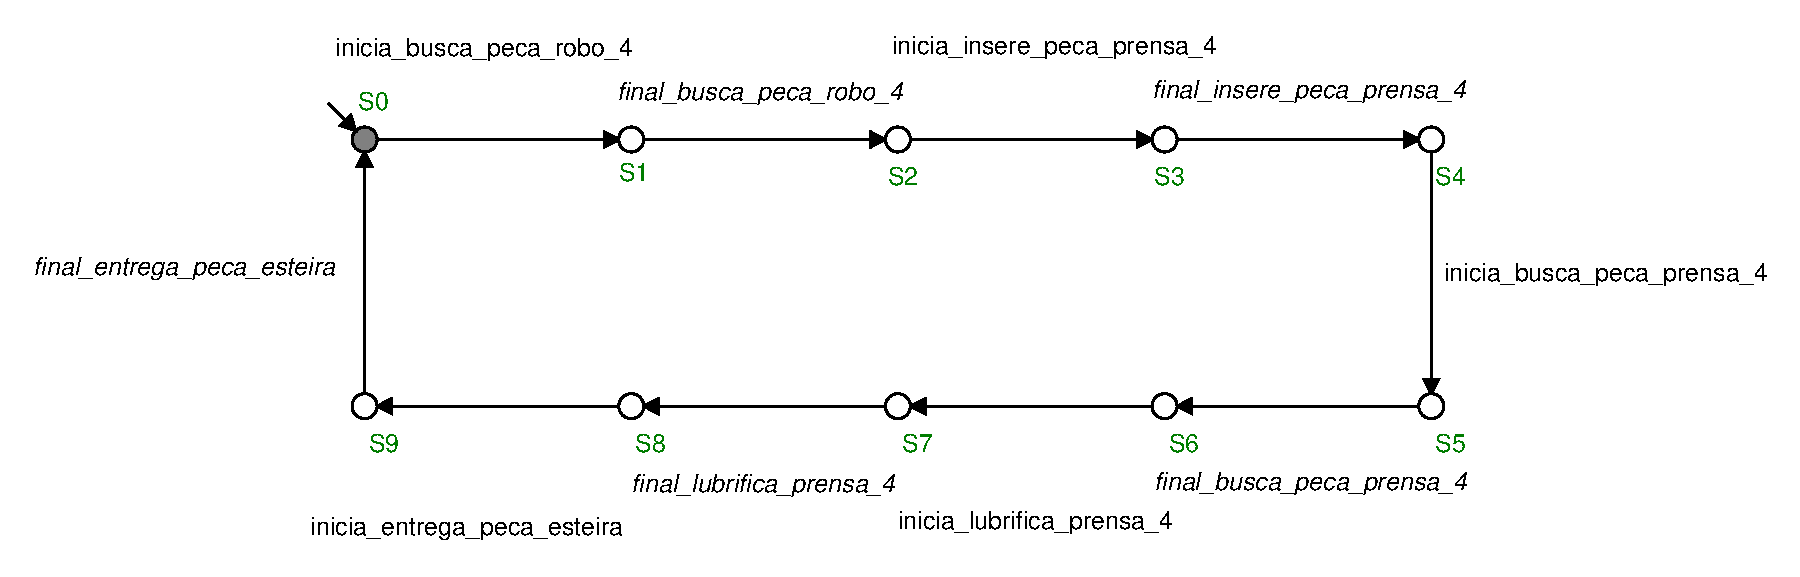
\includegraphics[width=0.9\textwidth]{imagens/robo_5.eps}
	\caption{Planta do robô 5.}\label{fig:robo5}
\end{figure}

Todas as quatro prensas funcionam da mesma maneira, tendo um acionador denotado por Bimanual, o qual ao ser acionado liga o motor fazendo com que essa movimente-se linearmente na vertical, subindo e descendo. As prensas possuem alguns sinais internos para identificar o posicionamento dessa, sendo eles:

\begin{enumerate}
	\item Ponto morto superior (PMS): este sinal é enviado quando o martelo da prensa esta na parte superior;
	
	\item Ponto morto inferior (PMI): este sinal é enviado quando o martelo da prensa esta na parte inferior;
	
	\item Bimanual: sinal para acionar o motor da prensa e permitir ela de realizar o movimento;
	
	\item Após início de operação pode ocorrer algum evento de interrupção e o retorno da interrupção leva a prensa para um estado seguro inicial.
\end{enumerate}

A planta para as prensas é mostrada na Figura \ref{fig:prensa}, onde verifica-se os eventos de início e final de operação da prensa e, também os eventos relacionados com a interrupção. Vale destacar que é considerado um ciclo completo de trabalho da prensa quando esta passa do $PMS \to PMI \to PMS$.

\begin{figure}[H]%
	\centering
	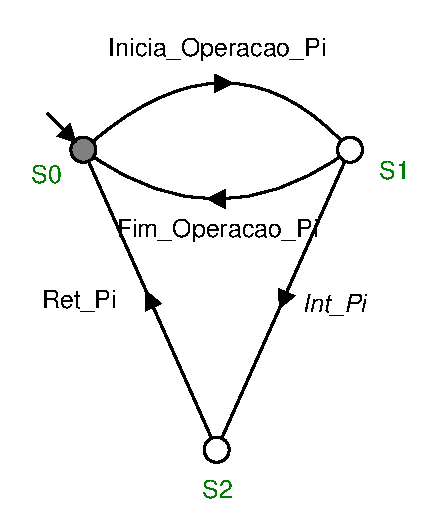
\includegraphics[width=0.6\textwidth]{imagens/Prensa.eps}
	\caption{Planta da prensa.}
	\label{fig:prensa}
\end{figure}


\subsection{Especificações}
A seção que se segue apresenta as especificações propostas para coordenar as ações entres as suplantas para criar o fluxo do processo de manufatura.

A especificação apresentada na figura \ref{fig:e0} direciona o robô 1 a retirar a chapa da mesa centralizadora (Retira\_Peca\_Mesa) após o sensor presente na mesa detectar existência de uma peça (Com\_Chapa). Enquanto a especificação apresentada na figura \ref{fig:e1} faz com que o robô 1 incie o processo de inserção da chapa na prensa 1 (Insere\_Peca\_P1) após ter à retirado da mesa centraliza e estar presente na garra (Retira\_Peca\_Mesa).

\begin{figure}[H]%
  \centering
  \begin{subfigure}[b]{0.45\textwidth}
      \centering
      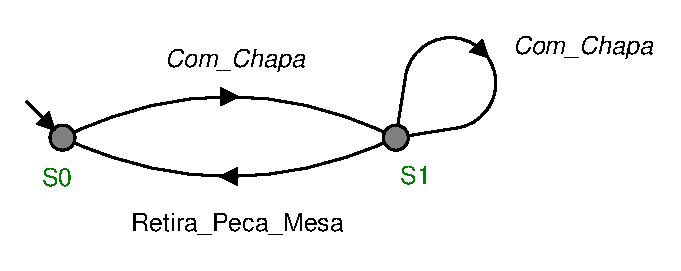
\includegraphics[width=\textwidth]{imagens/E0.eps}
      \caption{E0}
      \label{fig:e0}
  \end{subfigure}
  \hfill
  \begin{subfigure}[b]{0.45\textwidth}
      \centering
      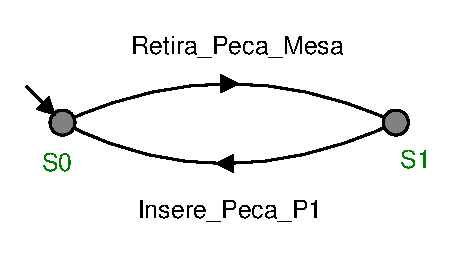
\includegraphics[width=\textwidth]{imagens/E1.eps}
      \caption{E1}
      \label{fig:e1}
  \end{subfigure}
  \caption{Especificações 0 e 1}
  \label{fig:e01}
\end{figure}

Na figura \ref{fig:e2} a especificação libera a prensa 1 iniciar a operação (Inicia\_Operacao\_P1) após o robô 1 finalizar a inserção da chapa e ter retornado à uma posição segura (Retorno\_P1). Na especificação apresentada na figura ref{fig:e3} modela a situação de \textit{overflow} da prensa 1, pois libera uma nova inserção (Insere\_Peca\_P1) somente após a retirada da peça pelo robô 2 (Retirou\_peca\_P1).

\begin{figure}[H]%
  \centering
  \begin{subfigure}[b]{0.45\textwidth}
      \centering
      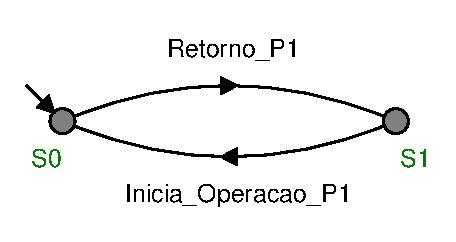
\includegraphics[width=\textwidth]{imagens/E2.eps}
      \caption{E2}
      \label{fig:e2}
  \end{subfigure}
  \hfill
  \begin{subfigure}[b]{0.45\textwidth}
      \centering
      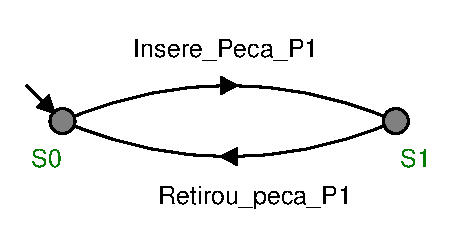
\includegraphics[width=\textwidth]{imagens/E3.eps}
      \caption{E3}
      \label{fig:e3}
  \end{subfigure}
  \caption{Especificações 2 e 3}
  \label{fig:e23}
\end{figure}

A especificação apresentada na figura \ref{fig:e4} limita o robô 2 a fazer retirada da peça na prensa 1 (Retira\_Peca\_P1) após o final da operação (Fim\_Operacao\_P1). A figura \ref{fig:e5} inibe o robô 2 de iniciar o processo de inserção na prensa 2 (Insere\_Peca\_P2) antes que a peça esteja presente na garra (Retira\_Peca\_P1).

\begin{figure}[H]%
  \centering
  \begin{subfigure}[b]{0.45\textwidth}
      \centering
      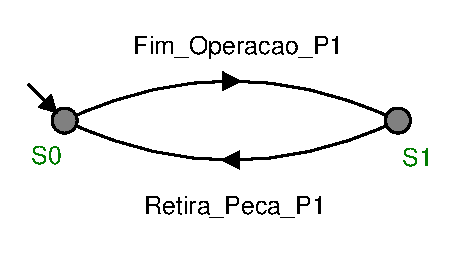
\includegraphics[width=\textwidth]{imagens/E4.eps}
      \caption{E4}
      \label{fig:e4}
  \end{subfigure}
  \hfill
  \begin{subfigure}[b]{0.45\textwidth}
      \centering
      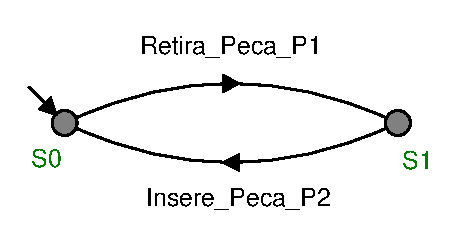
\includegraphics[width=\textwidth]{imagens/E5.eps}
      \caption{E5}
      \label{fig:e5}
  \end{subfigure}
  \caption{Especificações 4 e 5}
  \label{fig:e45}
\end{figure}

A especificação apresentada na figura \ref{fig:e6} libera a prensa 2 para iniciar a operação (Inicia\_Operacao\_P2) após o robô 2 finalizar a inserção e retornar à uma posição segura (Retorno\_P2). E a especificação apresentada na figura \ref{fig:e7} modela a situação de \textit{overflow} da prensa 2 e libera uma nova inserção (Insere\_Peca\_P2) somente após a retirada da peça pelo robô 3 (Retirou\_Peca\_P2).

\begin{figure}[H]%
  \centering
  \begin{subfigure}{0.45\textwidth}
      \centering
      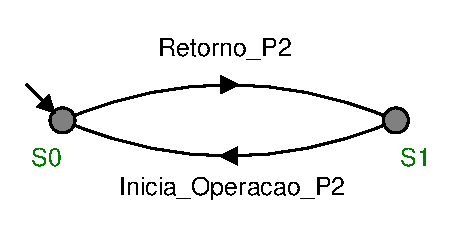
\includegraphics[width=\textwidth]{imagens/E6.eps}
      \caption{E6}
      \label{fig:e6}
  \end{subfigure}
  \hfill
  \begin{subfigure}{0.45\textwidth}
      \centering
      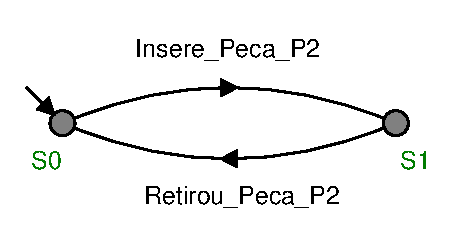
\includegraphics[width=\textwidth]{imagens/E7.eps}
      \caption{E7}
      \label{fig:e7}
  \end{subfigure}
  \caption{Especificações 6 e 7}
  \label{fig:e67}
\end{figure}

A especificação apresentada na figura \ref{fig:e8} limita o robô 3 a retirar peça da prensa 2 (Retira\_Peca\_P2) após o final da operação (Fim\_Operacao\_P2). E a especificação apresentada na figura \ref{fig:e9} limita o robô 3 a iniciar o processo de inserção na prensa 3 (Insere\_Peca\_P3) após a peça estar presente na garra (Retira\_Peca\_P2).

\begin{figure}[H]%
  \centering
  \begin{subfigure}{0.45\textwidth}
      \centering
      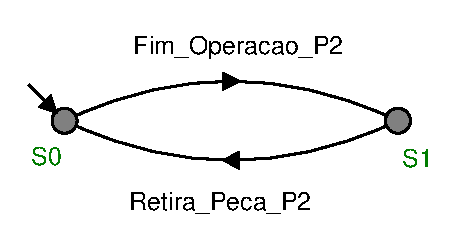
\includegraphics[width=\textwidth]{imagens/E8.eps}
      \caption{E8}
      \label{fig:e8}
  \end{subfigure}
  \hfill
  \begin{subfigure}{0.45\textwidth}
      \centering
      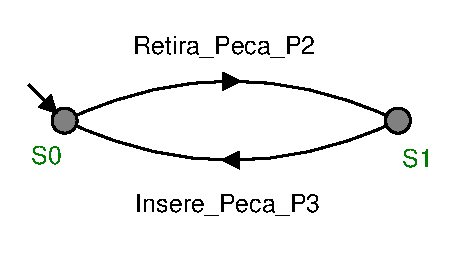
\includegraphics[width=\textwidth]{imagens/E9.eps}
      \caption{E9}
      \label{fig:e9}
  \end{subfigure}
  \caption{Especificações 8 e 9}
  \label{fig:e89}
\end{figure}

A especificação apresentada na figura \ref{fig:e10} permite que a prensa 3 inicie a operação (Inicia\_Operacao\_P3) após o robô 3 finalizar a inserção e estar em posição segura (Retorno\_P3).A especificação apresentada na figura \ref{fig:e11} é o modelo para \textit{overflow} da prensa 3 e libera uma nova inserção (Insere\_Peca\_P3) somente após a retirada da peça pelo robô 4 (Retira\_Peca\_P3).

\begin{figure}[H]%
  \centering
  \begin{subfigure}{0.45\textwidth}
      \centering
      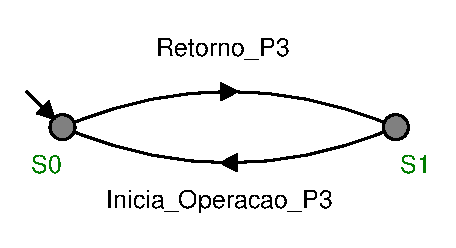
\includegraphics[width=\textwidth]{imagens/E10.eps}
      \caption{E10}
      \label{fig:e10}
  \end{subfigure}
  \hfill
  \begin{subfigure}{0.45\textwidth}
      \centering
      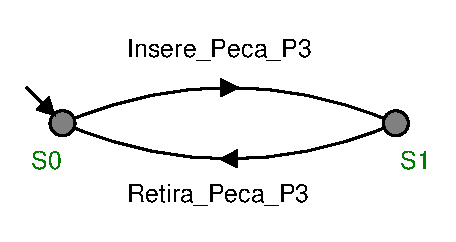
\includegraphics[width=\textwidth]{imagens/E11.eps}
      \caption{E11}
      \label{fig:e11}
  \end{subfigure}9
  \caption{Especificações 10 e 11}
  \label{fig:e1011}
\end{figure}

A especificação apresentada na figura \ref{fig:e12} limita o robô 4 a retirar peça da prensa 3 (Retira\_Peca\_P3) somente após o final da operação (Fim\_Operacao\_P3). A especificação apresentada na figura \ref{fig:e13} limita o robô 4 a iniciar o processo de entrega para robô 5 (Leva\_Peca\_R5) após a peça estar presente na garra (Retira\_Peca\_P3).

\begin{figure}[H]%
  \centering
  \begin{subfigure}{0.45\textwidth}
      \centering
      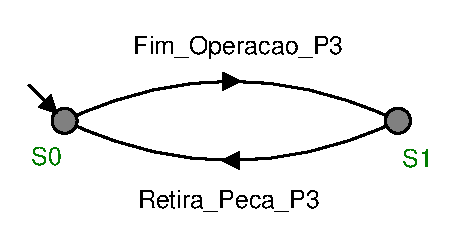
\includegraphics[width=\textwidth]{imagens/E12.eps}
      \caption{E12}
      \label{fig:e12}
  \end{subfigure}
  \hfill
  \begin{subfigure}{0.45\textwidth}
      \centering
      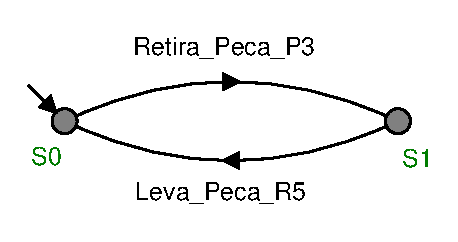
\includegraphics[width=\textwidth]{imagens/E13.eps}
      \caption{E13}
      \label{fig:e13}
  \end{subfigure}
  \caption{Especificações 12 e 13}
  \label{fig:e1213}
\end{figure}

A especificação apresentada na figura \ref{fig:e14} permite que a Prensa 4 inicie a operação (Inicia\_Operacao\_P4) após o robô 5 finalizar a inserção e estar em posição segura (Retorno\_P4).A especificação apresentada na \ref{fig:e15} limita o robô 5 a retirar peça da prensa 5 (Retira\_Peca\_P4) após o final da operação (Fim\_Operacao\_P4).

\begin{figure}[H]%
  \centering
  \begin{subfigure}{0.45\textwidth}
      \centering
      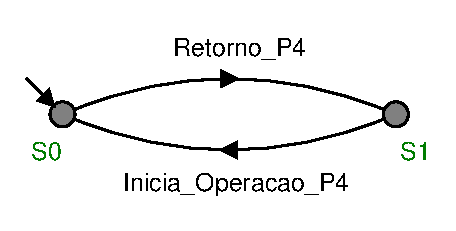
\includegraphics[width=\textwidth]{imagens/E14.eps}
      \caption{E14}
      \label{fig:e14}
  \end{subfigure}
  \hfill
  \begin{subfigure}{0.45\textwidth}
      \centering
      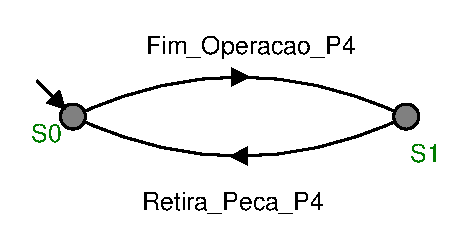
\includegraphics[width=\textwidth]{imagens/E15.eps}
      \caption{E15}
      \label{fig:e15}
  \end{subfigure}
  \caption{Especificações 14 e 15}
  \label{fig:e1415}
\end{figure}

A especificação apresentada na figura \ref{fig:e16} força robô 4 ao entregar uma peça (Leva\_Peca\_R5) aguarde o movimento do robô 5 de buscar a peça (Retira\_Peca\_R4).
A especificação apresentada na figura \ref{fig:e17} força o robô 4 a aguardar o retorno para a posição segura do robô 5 (Retorno\_R5) para retornar ao movimento de entrega de peça entre a prensa 4 e o robô 5 (Retirou\_Peca\_R4).

\begin{figure}[H]%
  \centering
  \begin{subfigure}{0.45\textwidth}
      \centering
      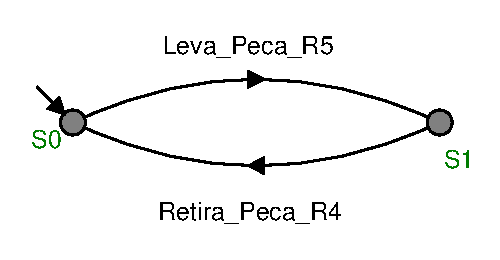
\includegraphics[width=\textwidth]{imagens/E16.eps}
      \caption{E16}
      \label{fig:e16}
  \end{subfigure}
  \hfill
  \begin{subfigure}{0.45\textwidth}
      \centering
      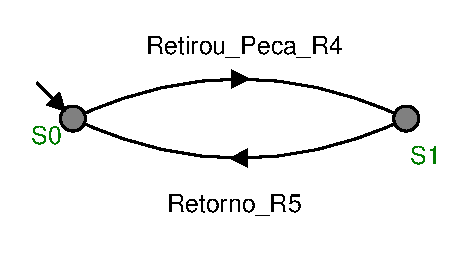
\includegraphics[width=\textwidth]{imagens/E17.eps}
      \caption{E17}
      \label{fig:e17}
  \end{subfigure}
  \caption{Especificações 16 e 17}
  \label{fig:e1617}
\end{figure}

A especificação apresentada na figura \ref{fig:e18} limita o robô 5 a iniciar o processo de inserção na prensa 4 (Insere\_Peca\_P4) após ter peça presente na garra (Retirou\_Peca\_R4).A especificação apresentada na \ref{fig:e19} permite que o robô 5 pegue uma nova peça do robô 4 (Retira\_Peca\_R4) após entregar a peça manufaturada na esteira (Retorno\_Esteira).

\begin{figure}[H]%
  \centering
  \begin{subfigure}{0.45\textwidth}
      \centering
      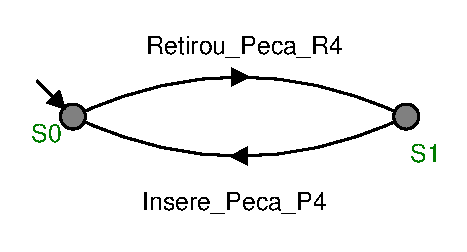
\includegraphics[width=\textwidth]{imagens/E18.eps}
      \caption{E18}
      \label{fig:e18}
  \end{subfigure}
  \hfill
  \begin{subfigure}{0.45\textwidth}
      \centering
      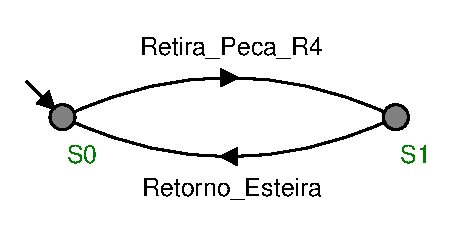
\includegraphics[width=\textwidth]{imagens/E19.eps}
      \caption{E19}
      \label{fig:e19}
  \end{subfigure}
  \caption{Especificações 18 e 19}
  \label{fig:e1819}
\end{figure}

\subsection{Solução modular de controle}
O software Supremica \cite{Supremica2020} disponibiliza a funcionalidade para verificação da modularidade dos modelos desenvolvidos.
A Figura \ref{fig:modulare0} apresenta o resultado da análise de modularidade para especificação E0 com as plantas, podemos verificar que a especificação realiza controle de eventos sobre o robô 1 e sobre Sensor Chapa sem ter dependência com outras plantas.

\begin{figure}[H]%
  \centering
  \includegraphics[width=0.8\textwidth]{imagens/modular-E0.eps}
  \caption{Estrutura modular para E0}\label{fig:modulare0}
\end{figure}

O processo de verificação de modularidade foi executado para todas as especificações individualmente. A tabela \ref{tab:modulos} apresenta o resultado para cada especificação e as respectivas plantas que se relacionam.
Foi verificado que o número máximo de interações de uma especificação é com duas plantas.

\begin{table}[h]%
\begin{center}
\begin{minipage}{0.5\textwidth}
\caption{Relações entre plantas e especificações}
\label{tab:modulos}
\begin{tabular}{@{}lll@{}}
  \toprule
  Especificação &  Planta 1 & Planta 2\\
  \midrule
  E0 & Sensor Chapa & Robô 1\\
  E1 & Robô 1 & \\
  E2 & Robô 1 & Prensa 1\\
  E3 & Robô 1 & Robô 2\\
  E4 & Robô 2 & Prensa 1\\
  E5 & Robô 2 & \\
  E6 & Robô 2 & Prensa 2\\
  E7 & Robô 2 & Robô 3\\
  E8 & Robô 3 & Prensa 2\\
  E9 & Robô 3 & \\
  E10 & Robô 3 & Prensa 3\\
  E11 & Robô 3 & Robô 4\\
  E12 & Robô 4 & Prensa 3\\
  E13 & Robô 4 & \\
  E14 & Robô 5 & Prensa 4\\
  E15 & Robô 5 & Prensa 4\\
  E16 & Robô 4 & Robo 5\\
  E17 & Robô 4 & Robo 5\\
  E18 & Robô 5 & \\
  E19 & Robô 5 & \\
  \botrule
\end{tabular}
\end{minipage}
\end{center}
\end{table}

\newpage

Utilizando-se da relação entre especificações e plantas foi calculado o supervisor não bloqueante e controlável modularmente para cada especificação.
A Tabela \ref{tab:supervisor} apresenta o número de estados, transições e eventos para cada supervisor modular que serão utilizados para obter o supervisor final.

\begin{table}[h]%
\begin{center}
\begin{minipage}{0.5\textwidth}
\caption{Supervisores Modulares}
\label{tab:supervisor}
\begin{tabular}{@{}llll@{}}
  \toprule
  Supervisor & Estados & Eventos & Transições\\
  \midrule
  Sup 0 & 8 & 7 & 23\\
  Sup 1 & 6 & 6 & 10\\
  Sup 2 & 24 & 10 & 73\\
  Sup 3 & 32 & 12 & 120\\
  Sup 4 & 24 & 10 & 73\\
  Sup 5 & 6 & 6 & 10\\
  Sup 6 & 24 & 10 & 73\\
  Sup 7 & 32 & 12 & 120\\
  Sup 8 & 24 & 10 & 73\\
  Sup 9 & 6 & 6 & 10\\
  Sup 10 & 24 & 10 & 73\\
  Sup 11 & 32 & 12 & 120\\
  Sup 12 & 24 & 10 & 73\\
  Sup 13 & 6 & 6 & 10\\
  Sup 14 & 30 & 12 & 98\\
  Sup 15 & 30 & 12 & 98\\
  Sup 16 & 40 & 14 & 159\\
  Sup 17 & 40 & 14 & 159\\
  Sup 18 & 9 & 8 & 18\\
  Sup 19 & 9 & 8 & 18\\
  %\midrule
  %\textbf{Final} & & &\\
  \botrule
\end{tabular}
\end{minipage}
\end{center}
\end{table}

\newpage

Por limitação computacional não foi possível realizar a composição de todos os supervisores para obtenção do controlador final, isso se deu devido à explosão do número de estados.
